%%% fs-seim-typical - Typical solutions

\label {fs-typical}

There are two common methods that are used to implement order-sensitive operators: in-order processing (IOP) \cite{Arasu:2006:CCQ:1146461.1146463} \cite{Cranor:2003:GSD:872757.872838} \cite{hammad2004optimizing} and out-of-order processing (OOP)\cite{Li:2008:OPN:1453856.1453890}.

\subsection{IOP}

In IOP approach each operation enforces total order on elements. For example, union combines multiple streams into one, see the figure~\ref{iop}. Each input stream of the union is ordered, as predecessors must meet ordering constraint. If there is arrival time skew between input stream, the union must buffer the earlier stream to produce ordered output. Operators such as projection and selection apply function and propagate items down the stream without any additional buffering.

\begin{figure}[htbp]
  \centering
  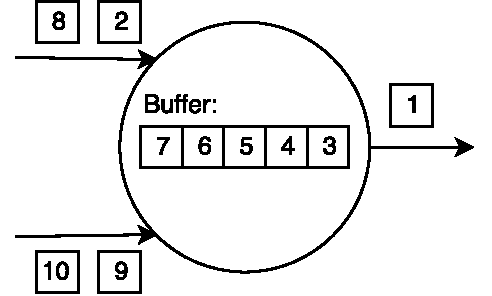
\includegraphics[width=0.30\textwidth]{pics/iop}
  \caption{IOP union operation. Due to delay of the upper stream operation must buffer elements}
  \label {iop}
\end{figure}

IOP is known to be memory demanding, to have unpredictable latencies and limited scalability.\cite{Li:2008:OPN:1453856.1453890}

\subsection{OOP}

OOP is an architecture of streaming systems that don't require order maintenance. To unblock blocking operations OOP systems use progress indicators such as punctuations \cite{Tucker:2003:EPS:776752.776780}, low watermarks \cite{Akidau:2013:MFS:2536222.2536229} or heartbeats \cite{Srivastava:2004:FTM:1055558.1055596}. Punctuations are periodically yielded by data sources and carry timestamp that promises that there won't be any elements older that punctuation's value. Punctuations are monotonic and data items between two consecutive punctuations can be arbitrarily reordered. Operations propagate them with respect to operation's semantics.

\begin{figure}[htbp]
  \centering
  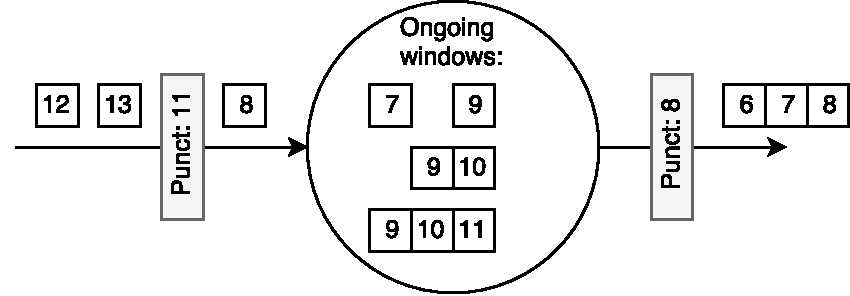
\includegraphics[width=0.48\textwidth]{pics/oop}
  \caption{OOP sliding window, range=3, slide=1. Operation must block lower window until next punctuation arrival }
  \label {oop}
\end{figure}

For example, window collects partial aggregates until punctuation that guarantees that there are no elements up the stream that belongs to the ongoing window. On punctuation's arrival it flushes completed windows and propagates punctuation to the next operation down the stream.

OOP resolves some of the downsides of IOP but it has several flaws. Even if the input stream is totally ordered, the operation must wait for the punctuation to guarantee it. In the figure~\ref{oop} bottom window is complete but must be blocked until the punctuation for item 11 arrives. Another issue is that periodical flushes can result in load bursts. This can lead to latencies increase. 
